\documentclass{article}
\usepackage[utf8]{inputenc}
\usepackage[spanish]{babel}
\usepackage{listings}
\usepackage{graphicx}
\graphicspath{ {images/} }
\usepackage{cite}

\begin{document}

\begin{titlepage}
    \begin{center}
        \vspace*{1cm}
            
        \Huge
        \textbf{PROCESAMIENTO DE IMÁGENES  }
            
        \vspace{0.5cm}
        \LARGE
        Parcial 2
            
        \vspace{1.5cm}
            
        \textbf{Sergio Alberto Giraldo  Salazar \\ Diego Fernando Urbano Palma }
        
        \vfill
            
        \vspace{0.8cm}
            
        \Large
        Departamento de Ingeniería Electrónica y Telecomunicaciones\\
        Universidad de Antioquia\\
        Medellín\\
        Septiembre de 2021
            
    \end{center}
\end{titlepage}

\tableofcontents
\newpage
\section{Análisis del problema}\label{intro}
En el presente parcial se nos pide dar una interpretación de una imagen donde se submuestrea o se sobremuestrea para que sea compatible con la matriz de leds que se va montar en TINKERCAD.
Con el presente proyecto se evidencian  las siguientes dificultades, como lo serian la interpretación de datos por parte del TINKERCAD.\\
Otra dificultad para el proyecto es entender las matrices de datos que nos van a mostrar en el camino, como lo es la matriz RGB la cual nos dan el color de cada pixel para poder generar un código que nos  submuestre o sobremuestre la imagen. \\Saber que es sobremuestreo  y submuestre ya que es el eje de la practica 2 que en este momento estamos presentando. \\
Manejar correctamente las librerías de Arduino para darle el color deseado a nuestros leds mostrando la imagen después de haber completado el los procesos para tratar una imagen.


\section{funcionamiento del circuito} \label{contenido}

\begin{figure}[h]
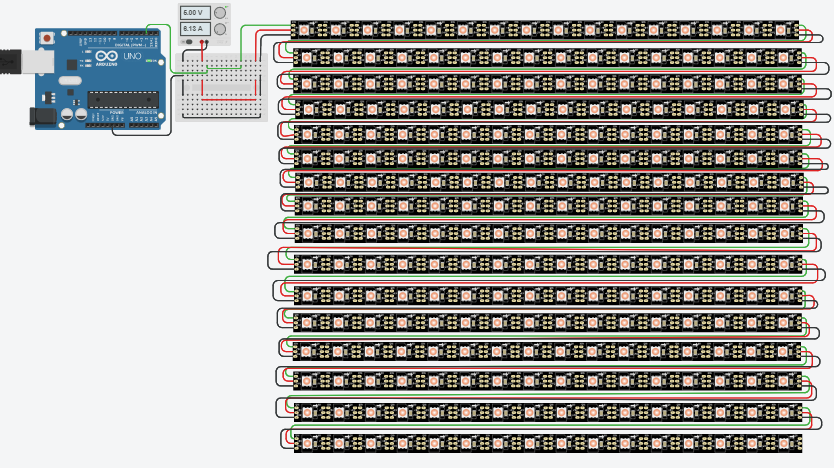
\includegraphics[width=10cm]{Simulación.png}
\centering
\caption{Matriz de leds}
\label{fig:matriz de leds}
\end{figure}

\label{contenio}
En la imagen se plantea una matriz de leds 16*16 donde el primer led a tomar en cuenta será el superior a la izquierda y de allí se ira avanzando hacia la derecha, decidimos tomar este orden para tener una mayor facilidad de compresión de como se ira reflejando los cambios en cada led.

\subsection{Codigo Prueba }
\begin{lstlisting}[language=arduino, label=codigo_ejemplo]
#include <Adafruit_NeoPixel.h>
#define LED_PIN    2
#define LED_COUNT 256

Adafruit_NeoPixel leds(LED_COUNT, LED_PIN, NEO_GRB + NEO_KHZ800);

void setup(){
  leds.begin();
  
  for (int i=0; i<LED_COUNT;i++){
  leds.setPixelColor(i,207, 97, 62);
  }

  leds.show();
  
}

void loop()
{
}
\end{lstlisting}
\section{Plantiamiento de soluciones }

\subsection{Información de la imagen  }

Para poder manejar la información de la imagen en el tinkercard lo que tenemos que hacer es por medio de C++ transformar los datos de cada pixel en una matriz, modificarla y pegar dicha matriz como constantes en el simulador para que de esta manera podamos manejar la información de cada uno de los pixeles, como se muestra en el pseudo código \ref{codigo_ejemplo}. 
\begin{lstlisting}[language=C++, label=codigo_ejemplo]

// Incluimos las librerias necesarias para leer
//la imagen y podemos realizar nuestro codigo
#include <iostream>
#include "QImage"
#include "string.h"
#include "fstream"
using namespace std;

int main()
{
    ///////// LECTURA DE PIXELES DE LA IMAGEN //////////
//declaramos las clases para la lectura de imagen
// y la de manipulacion de archivos de texto
    QImage imagen("direccion de la imagen ");
    fstream matriz("nombre del archivo de texto", fstream::app);
    unsigned InfLeds[3][16][16], azul,verde,rojo;
    string cadena;
// se hace una cadena de for para que se se obtenga
//la informacion de cada una de los pixeles de la imagen

    for(iterador <= altura de la imagen)
    {
        for(iterador<= ancho de la imagen)
        {

           InfLeds[0][iterador altura][iterador ancho]=azul;
           InfLeds[1][iterador altura][iterador ancho]=verde;
           InfLeds[2][iterador altura][iterador ancho]=rojo;
        }
    }


 /////////////////////////////////////////////////////////////////////////////////////////

    /// ingresar datos al txt ///
    for(iterador <= altura de la matriz de leds)
    {   cadena=cadena+"[";
        for(iterador<= ancho de la matriz de leds)
        {

           cadena=cadena+"azul,rojo,verde";
           matriz<<cadena;

        }
         cadena=cadena+"]";
    }



    return 0;
}
\end{lstlisting}

\subsection{sobremuestreo} \label{contenido}
El sobre muestreo según la definición dada en clase, es agarrar una imagen de una resolución baja o de poca densidad de pixeles y mediante un procedimiento ir aumentando la densidad   de la matriz, subiendo por ende la calidad.\\\\
Para cumplir ese procedimiento y mejorar la calidad de la imagen, vamos a tener en cuenta el  método de aumentar  separando los pixeles e ir rellenando los espacios con colores semejantes que vayan escalando al color del pixel vecino como se muestra en la imagen. 

\begin{figure}[h]
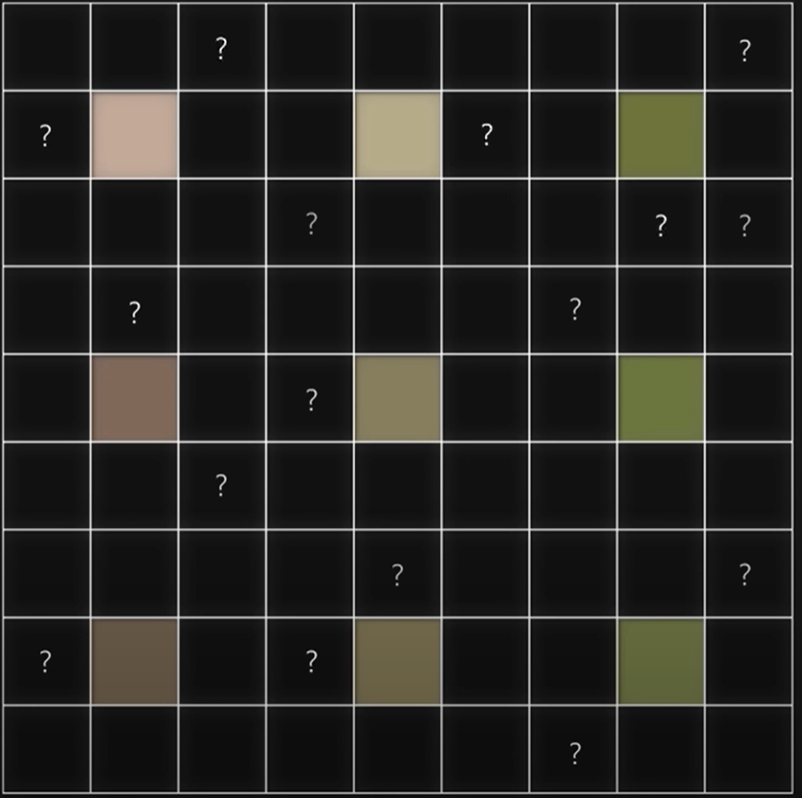
\includegraphics[width=4cm]{matriz_a_llenar.png}
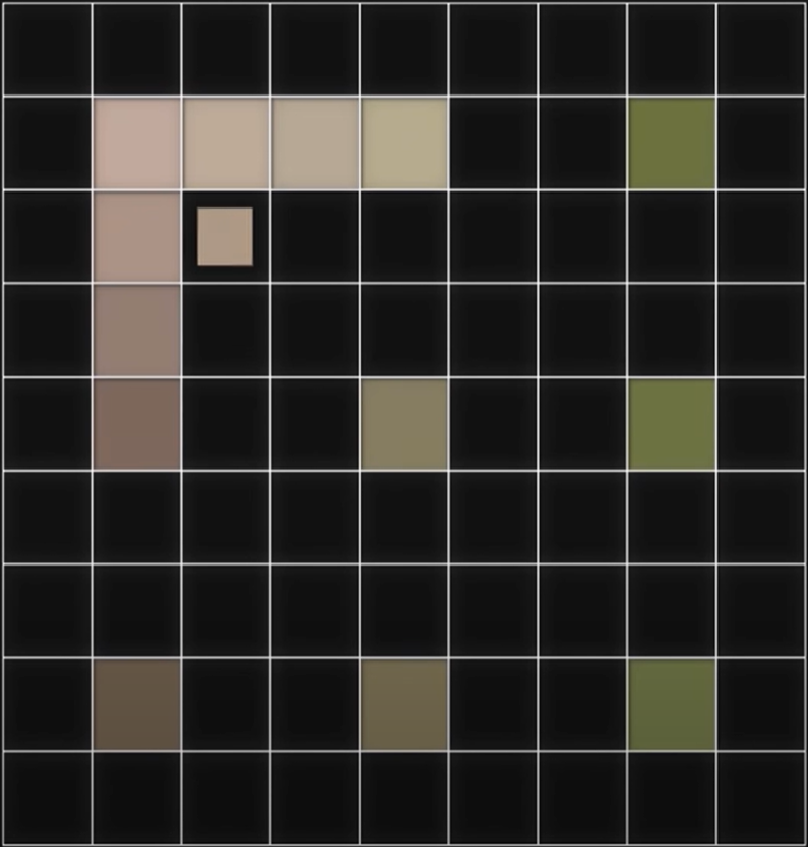
\includegraphics[width=4cm]{llenado_de_matriz.png}
\centering
\caption{separacion de pixeles}
\label{fig:matriz de leds}
\end{figure}






\subsection{sub muestreo }\label{contenido}
Una estrategia para reducir el espacio entre pixeles sería, asignándole a los nuevos pixeles el gradiente o extrapolación matemática de los pixeles eliminados combinando proporcionalmente las intensidades de los pixeles que conocemos, si esto lo hacemos con todos los pixeles obtendríamos una imagen con un tamaño reducido que no pierde mucho la información que contenía la imagen. \\\\
Otra estrategia para reducir el tamaño de la imagen seria tomar varios pixeles con valores en RGB que tengan el mismo valor de píxel, para posteriormente tomar el píxel central y eliminar los del alrededor para tener la misma información inicial en una cantidad menor de pixeles.\\\\

\begin{figure}[h]
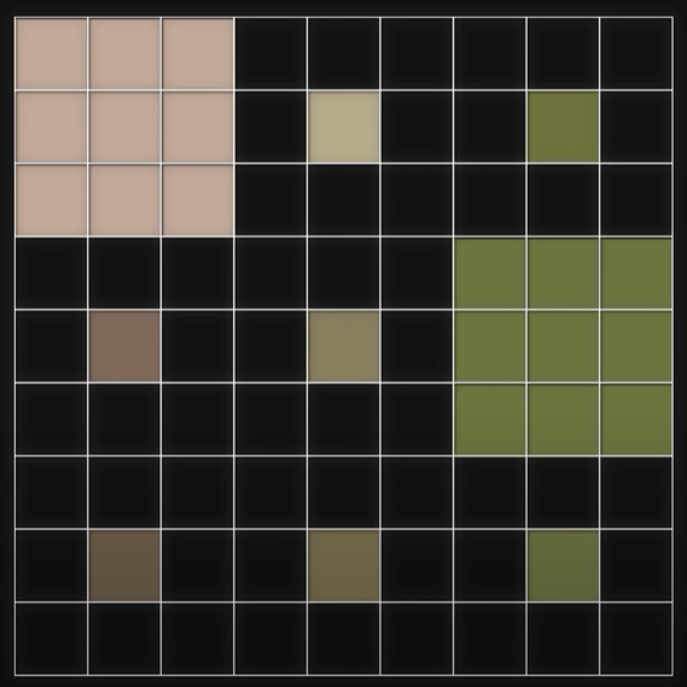
\includegraphics[width=6cm]{MatrizCompleta.png}
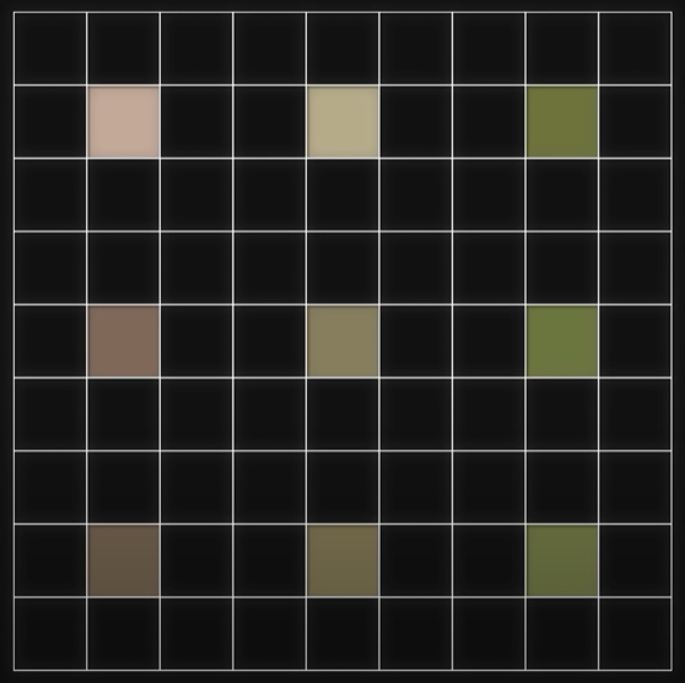
\includegraphics[width=6cm]{MatrizReducida.png}
\centering
\caption{Redución en el numero de pixeles}
\label{fig:matriz de leds}
\end{figure}

\subsection{Adecuacion de tamaño }
\begin{figure}[h]
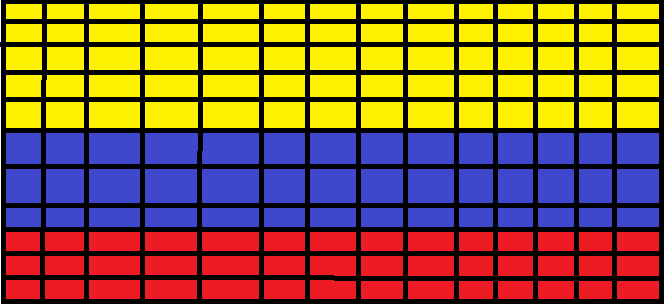
\includegraphics[width=6cm]{bandera_pixel.png}
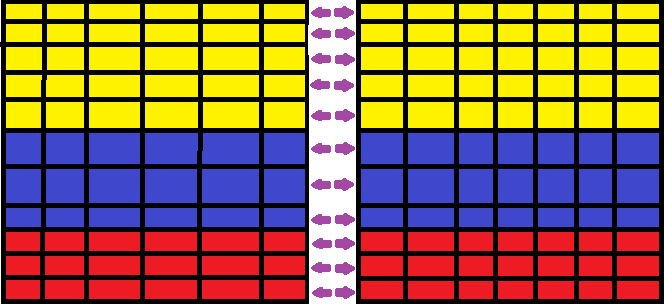
\includegraphics[width=6cm]{eliminar_pixel.png}
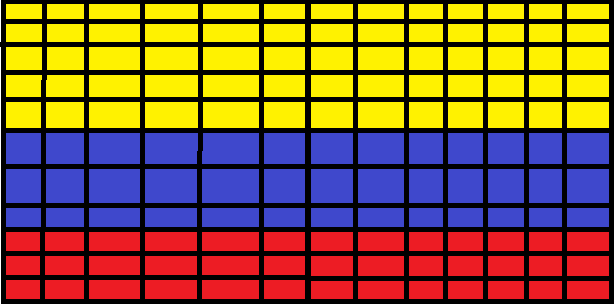
\includegraphics[width=5.5cm]{acomodar.png}
\centering
\caption{cortar pixeles iguales}
\label{fig:matriz de leds}
\end{figure}
Para el presente trabajo de procesamiento de imágenes para posteriormente implementarlo en el Tinkercard y por ende reproducirlo tenemos que adecuar la imagen procesada para que sea cuadrada según el circuito montado.\\
El código a implementar para solucionar el problema de la imagen no cuadrada o que no encaje con el circuito consiste en  ir escaneando pixel por pixel y encontrar  líneas que tengan información igual a ambos lados de donde se esté escaneando  e ir eliminándola hasta obtener el tamaño deseado y si la imagen no tiene información repetida se ira promediando el color con los pixeles vecinos y de esta manera ir acortando la imagen hasta quedar con el tamaño deseado.

\newpage 

\section{Codigo}
\subsection{Clases}


    class tamano
    {
    protected:

    public:
        unsigned **cambio;
        unsigned long long alto, ancho ;
        tamano(unsigned alto,unsigned ancho);

    };

    class submuestreo:protected tamano
    {
    private:

    public:
        // toma un conjunto de pixeles para comprobar si los valores RGB se repiten
        void anilisis();
        //toma los valores RGB de un conjunto de pixeles y entregue un pixel con el promedio de estos valores RGB
        void promediocolor();
        //elimina información duplicada para reducir el tamaño de la matriz para que quede cuadrada
        void eliminar();

    };
    
    
    class sobremuestreo:protected tamano
    {
    private:
                
    public:
        // toma un conjunto de pixeles para comprobar si los valores RGB se repiten
        void anilisis();
        //toma los valores RGB de un conjunto de pixeles y entregue un pixel con el promedio de estos valores RGB
        void promediocolor();
        //elimina información duplicada para reducir el tamaño de la matriz para que quede cuadrada
        void eliminar();

    };


    return 0;


\begin{lstlisting}[language=C++, label=codigo clases]


















\end{lstlisting}
\bibliographystyle{IEEEtran}
\bibliography{references}

\end{document}
